% Unofficial University of Cambridge Poster Template
% https://github.com/andiac/gemini-cam
% a fork of https://github.com/anishathalye/gemini
% also refer to https://github.com/k4rtik/uchicago-poster

\documentclass[final]{beamer}

% ====================
% Packages
% ====================

\usepackage[T1]{fontenc}
\usepackage{lmodern}
\usepackage[orientation=portrait,size=a1,scale=1.2]{beamerposter}
\usetheme{gemini}
\usecolortheme{cam}
\usepackage{graphicx}
\usepackage{booktabs}
\usepackage[numbers]{natbib}
\usepackage{tikz}
\usepackage{pgfplots}
\pgfplotsset{compat=1.14}
\usepackage{anyfontsize}
\usepackage{amsmath}

\setcitestyle{numbers}
\bibliographystyle{abbrvnat}
% ====================
% Lengths
% ====================

% If you have N columns, choose \sepwidth and \colwidth such that
% (N+1)*\sepwidth + N*\colwidth = \paperwidth
\newlength{\sepwidth}
\newlength{\colwidth}
\setlength{\sepwidth}{0.005\paperwidth}
\setlength{\colwidth}{0.45\paperwidth}

\newcommand{\separatorcolumn}{\begin{column}{\sepwidth}\end{column}}

% ====================
% Title
% ====================

\title{\huge A Survey of Explainable AI (XAI) Methods for Convolutional Neural Networks}

\author{\large Antonio Fernando Silva e Cruz Filho \inst{1} \and João Gabriel Andrade de Araujo Josephik\inst{1} \and Prof. Dr. Nina S. T. Hirata}

\institute[shortinst]{\inst{1} Institute of Mathematics and Statistics}

% ====================
% Footer (optional)
% ====================

\footercontent{
  \href{http://bit.ly/3V8BNdc}{http://bit.ly/3V8BNdc} \hfill
  Capstone Project - IME/USP \hfill
  fernandof.cruz@usp.br/joao.gabrielaaj@usp.br}
% (can be left out to remove footer)

% ====================
% Logo (optional)
% ====================

% use this to include logos on the left and/or right side of the header:
% \logoright{\includegraphics[height=7cm]{logo1.pdf}}
% \logoleft{\includegraphics[height=7cm]{logo2.pdf}}

\newcommand{\argmin}{\mathop{\mathrm{arg\,min}}}

% ====================
% Body
% ====================

\begin{document}

% Refer to https://github.com/k4rtik/uchicago-poster
% logo: https://www.cam.ac.uk/brand-resources/about-the-logo/logo-downloads
% \addtobeamertemplate{headline}{}
% {
%     \begin{tikzpicture}[remember picture,overlay]
%       \node [anchor=north west, inner sep=3cm] at ([xshift=0.0cm,yshift=1.0cm]current page.north west)
%       {\includegraphics[height=4.5cm]{logos/cambridge-reversed-color-logo.eps}}; 
%     \end{tikzpicture}
% }

% Acredito que podemos usar uma estrutura assim:

% Introduction
% Feature Visualization
% Saliency Maps
% LIME in Images
% Experiments
% Conclusion
% References

\begin{frame}[t]
\begin{columns}[t]
\separatorcolumn

\begin{column}{\colwidth}

  \begin{block}{Introduction}

    As artificial intelligence (AI) becomes part of critical fields like healthcare, finance, and autonomous vehicles, it’s important to understand how these systems make decisions. This is where Explainable AI (XAI) comes in. XAI helps make AI models, which are often complex, easier to understand and interpret. This ensures that AI systems are trusted and used responsibly.

    Neural networks are powerful tools for tasks like recognizing images or making predictions. However, they are often seen as "black boxes" because it’s hard to explain how they reach their decisions. This lack of clarity can be a problem in areas where understanding the reason behind a decision is as important as the result itself.
    \begin{columns}
      
      \begin{column}{0.6\textwidth}
        \begin{figure}
          \centering
          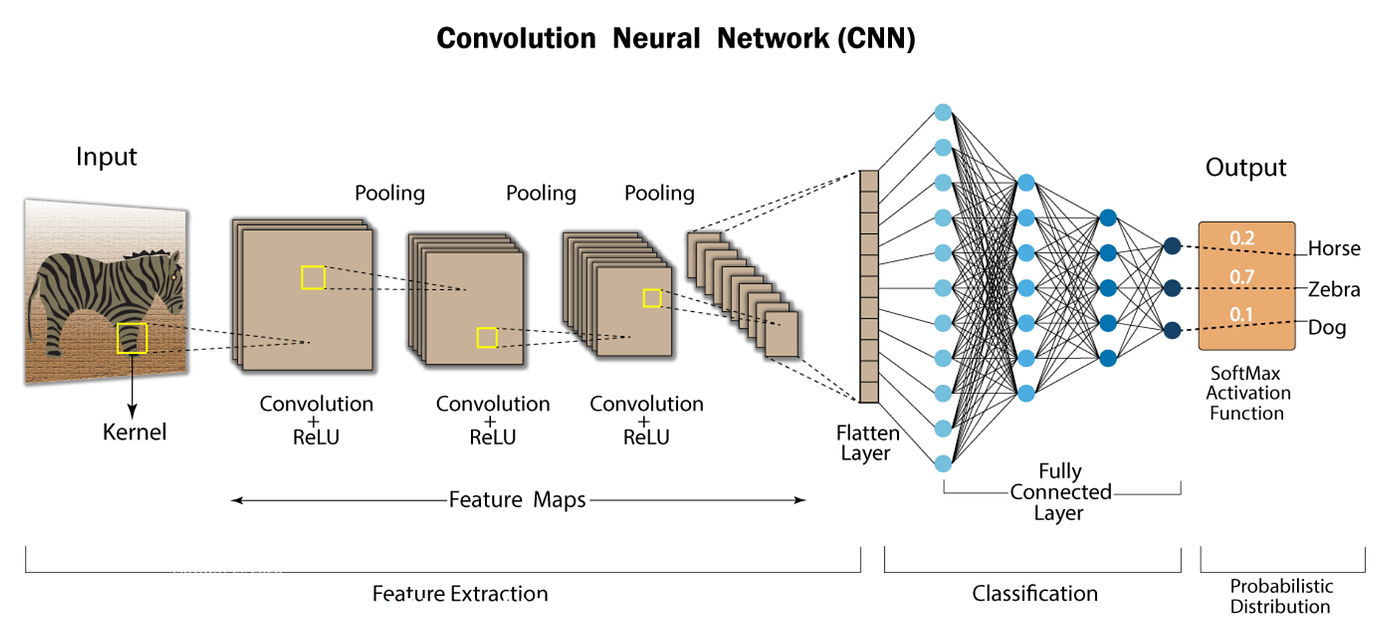
\includegraphics[width=\linewidth]{images/cnns.png}
          \caption{Convolutional Neural Network Architecture}
        \end{figure}
      \end{column}

      \begin{column}{0.4\textwidth}        
        
        \textbf{Convolutional Neural Networks (CNNs)} are neural networks designed for image and spatial data. They process parts of an image (like edges or textures) and combine these features to make decisions, making them ideal for tasks like face or object recognition.
        However, CNNs are also complex, and it can be hard to tell what they are focusing on and why. 
        XAI tools can help with this by showing how the CNN works step by step.
      \end{column}
    
    \end{columns}
    We will explore methods such as Feature Visualization, Saliency Maps, and LIME focused on explaining black-box image models like CNNs, aiming to create more robust, reliable, and less biased networks.
  \end{block}

  \begin{block}{Feature Visualization}
    CNNs can learn abstract features and concepts from images. 
    One can use techniques such as Feature Visualization to visualize the learned features by maximizing a network's neuron (or a set of neurons) value.
    This technique, called \emph{Activation Maximization}, can be modeled by the formula below, using the \emph{Gradient Ascent} method:
    \[x_{t + 1} = x_{t} + \mu \;\frac{\partial a(\theta, x_t)}{\partial x_t}\]
    Where \(x_t\) represents an image at iteration \(t\), \(\mu\) represents a tunable hyperparameter and the function \(a\) represents the forward pass of a unit in a Neural Network with parameters \(\theta\).
    
    By defining \(x_0\) as a specific image or just random noise, one can create \emph{dreamy-like} \cite{deepdream} images representing that will maximize a certain set of neurons of a Network.
    \begin{columns}  
      \begin{column}{0.5\textwidth}
        \begin{figure}
          \centering
          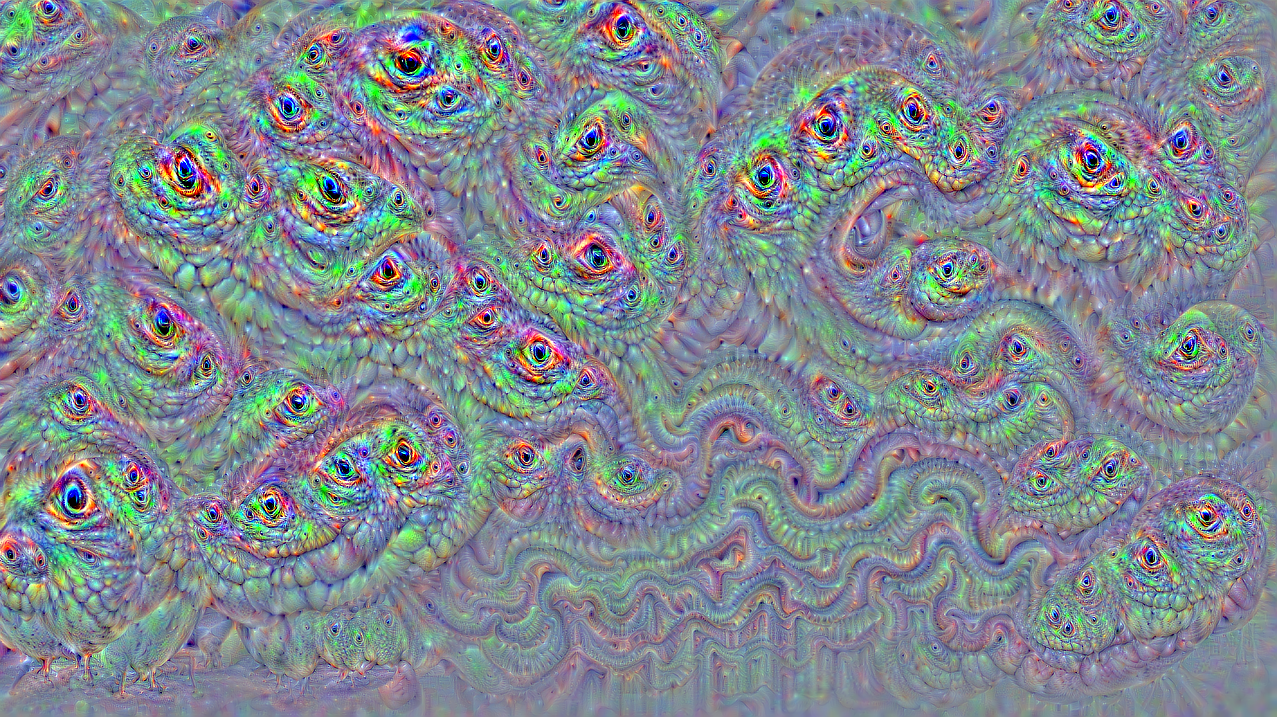
\includegraphics[width=\linewidth]{images/random_image_dream.png}
          \caption{Feature Visualization of CNN VGG16 using a random image}
        \end{figure}  
      \end{column}

      \begin{column}{0.5\textwidth}
        \begin{figure}
          \centering
          \includegraphics[width=\linewidth]{images/ime-dream.png}
          \caption{Feature Visualization of CNN VGG16 using a photo of IME-USP}
        \end{figure}
      \end{column}
      
    \end{columns}

    By close inspection in both images, one can notice that certain characteristic features like animal's eyes and dog's faces emerge,
    showing that the network learned those representations and certain layers are maximized by the presence of those features in images.
  \end{block}

  \begin{block}{GradCAM}

    At the last convolutional layer of a network, there are multiple channels representing extracted features from the image. Those features may be of multiple natures, such as presence of certain objects, simmetry, contrast, etc. By inspecting those channels, we can get an insight into what information the network is using to make its decision.

    The problem is: how can we know which channels are being useful to the decision? GradCAM solves this by averaging the feature maps weighted by the \textbf{gradient with regard to the output}. After that, we filter out negative influences by passing the output through the ReLU function. We can then resize the resulting map to the same size and overlay it over the original image to inspect the results.
    
    \begin{columns}  
      \begin{column}{0.5\textwidth}
        \begin{figure}
          \centering
          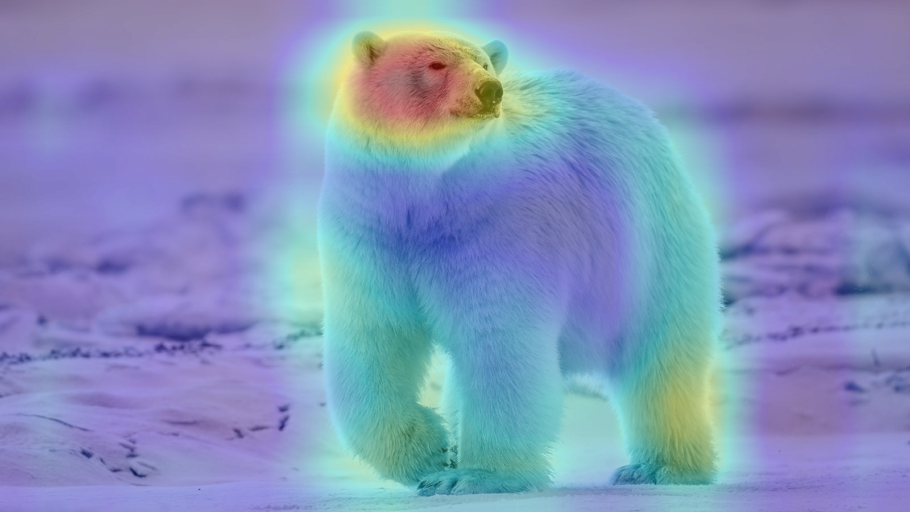
\includegraphics[width=\linewidth]{images/GC_ursopolar.png}
          \caption{GradCAM of a polar bear passed though ResNET. Network classification: polar bear, Ursus maritimus.}
        \end{figure}  
      \end{column}

      \begin{column}{0.5\textwidth}
        \begin{figure}
          \centering
          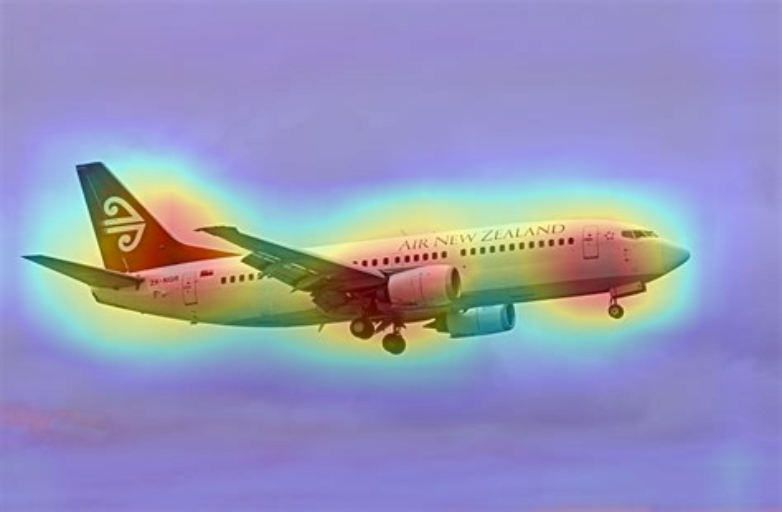
\includegraphics[width=\linewidth]{images/GC_aviao.png}
          \caption{GradCAM of a airplane passed though ResNET. Network classification: airliner}
        \end{figure}
      \end{column}
      
    \end{columns}
  \end{block}

  \begin{alertblock}{A highlighted block}

    This block catches your eye, so \textbf{important stuff} should probably go
    here.

    Curabitur eu libero vehicula, cursus est fringilla, luctus est. Morbi
    consectetur mauris quam, at finibus elit auctor ac. Aliquam erat volutpat.
    Aenean at nisl ut ex ullamcorper eleifend et eu augue. Aenean quis velit
    tristique odio convallis ultrices a ac odio.
  \end{alertblock}

\end{column}

\separatorcolumn

\begin{column}{\colwidth}

  \begin{block}{LIME in Images}

    LIME (Local interpretable model-agnostic explanations) is a technique to explain a complex model's decisions 
    by creating a simpler explainable model based on the complex model. A LIME model can be defined by the expression bellow:
    
    \[g^*(x) = \argmin_{g} L(f, g, \pi_x) + \Omega(g)\]
    
    Where \(L\) is a loss function to compare the simpler model performance with the complex model performance in the region close to \(x\), defined by \(\pi_x\). 
    \(\Omega\) is a function that returns a \textit{complexity metric} for a simple model \(g\).

    LIME can be used in images to create masks that represent areas that were more important for a model's decision.
    
    \begin{columns}
      \begin{column}{0.2\textwidth}
        \begin{figure}
          \centering
          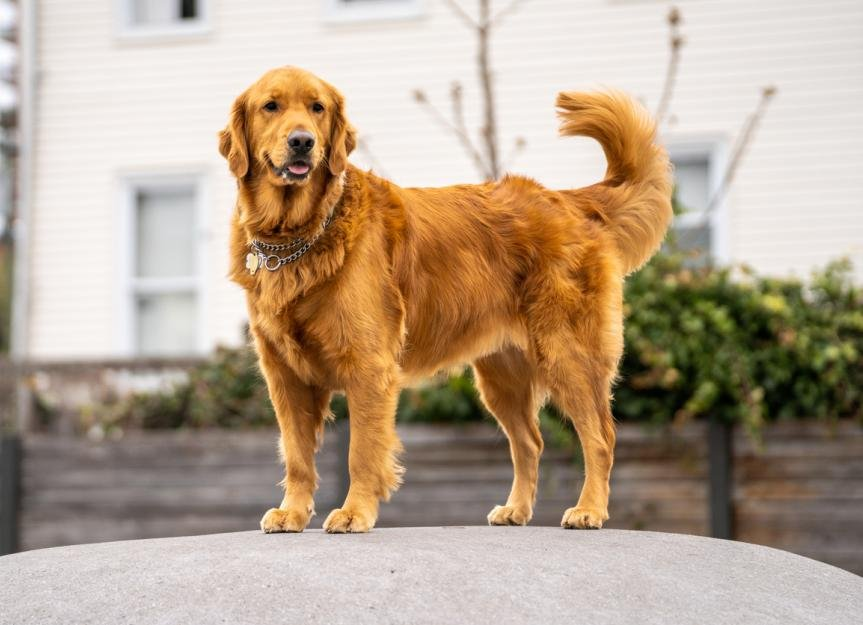
\includegraphics[width=0.85\linewidth]{images/dog.jpeg}
          \caption{Original Image}
        \end{figure} 
      \end{column}

      \begin{column}{0.2\textwidth}
        \begin{figure}
          \centering
          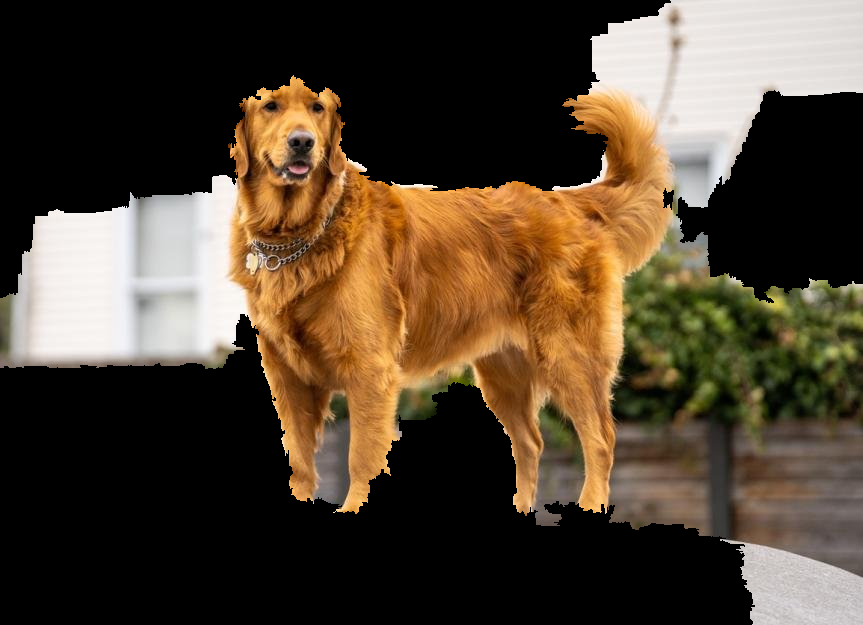
\includegraphics[width=0.85\linewidth]{images/lime.png}
          \caption{Masked image using LIME}
        \end{figure}
      \end{column}

    \end{columns}


  \end{block}

  \begin{block}{Experiments}
    We can check a network's robustness empirically by applying different kinds of filters 
    to an image and verifying changes in predictions and changes in focus regions using GradCAM.
    For example, here, we applied a brightness shift in a Red Fox image to check prediction and GradCAM variation in ResNet18:

    \begin{figure}
      \centering
      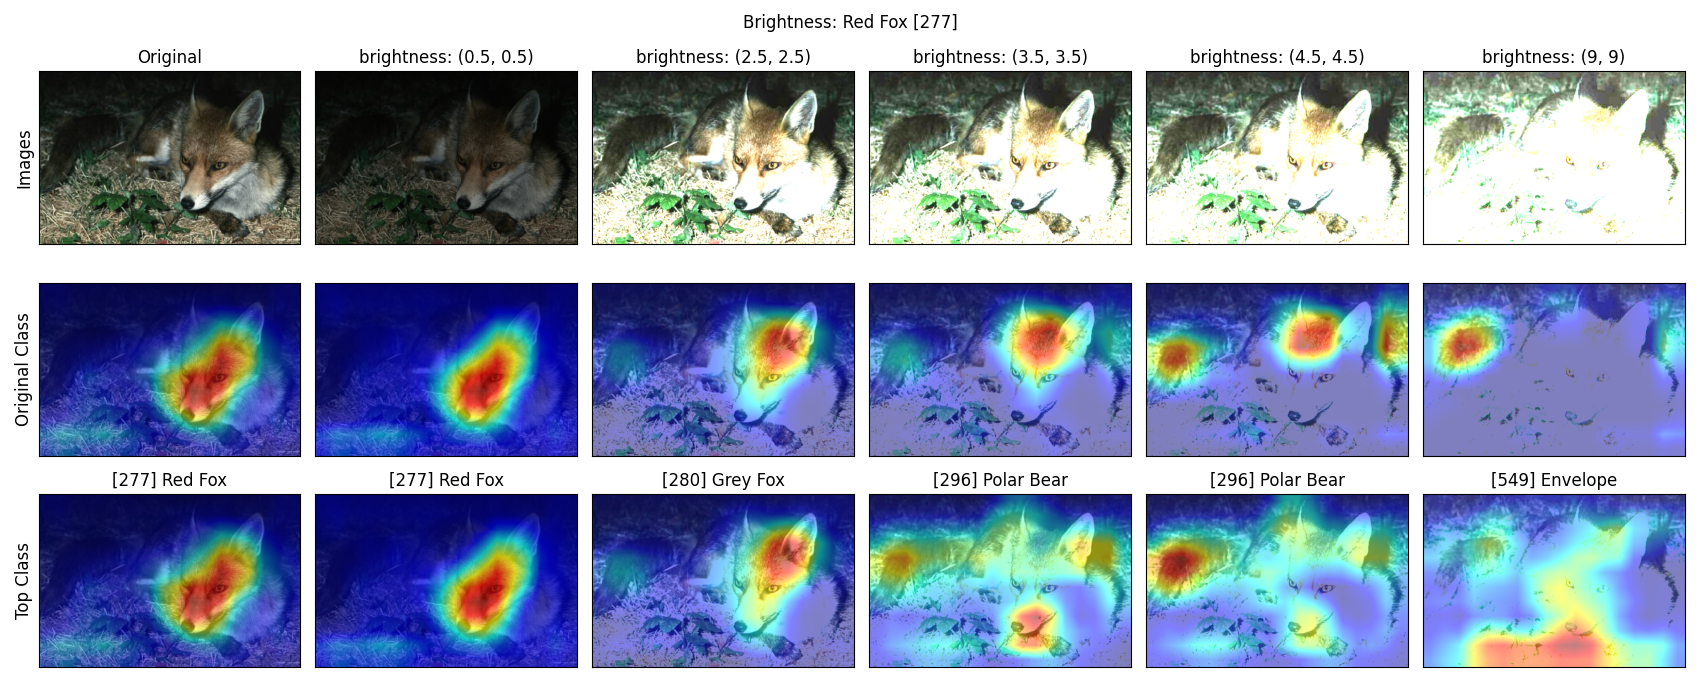
\includegraphics[width=0.96\linewidth]{images/fox-grad-cam-exp.png}
      \caption{Effect of brightness variation of a Red Fox image in ResNet18 Model}
    \end{figure}

    A clear correlation between white objects and a high presence of the color white in the image is reported 
    (predictions change to \textit{Polar Bear} or \textit{Envelope} in really bright images).
    Also, the GradCAM shows that, when the image is highly occluded by brightness, the fox's face is almost unrecognizable, 
    making the model \textit{"pay attention"} to the animal's tail, since this feature is still recognizable in this high brightness setting.
  \end{block}

  \begin{block}{Conclusion}

    Explainability tools like Feature Visualization, GradCAM and LIME enhance transparency by revealing how models make predictions. 
    This helps identify biases, debug issues, and build trust, ensuring AI systems are reliable and accountable.
  \end{block}

  \begin{block}{References}
    \nocite{*}
    \bibliography{bibliography}

  \end{block}

\end{column}

\end{columns}
\end{frame}

\end{document}
